\chapter{Gas Laws}
Unlike liquids, gasses are easily compressible.  Thus, the compressibility of the gasses must be taken into account when discussing how the gasses behave in relation to temperature and pressure.   There are four terms that must be defined with relation to gasses:
\begin{itemize}
	\item An \textbf{\textit{adiabatic}} \index{Adiabatic} process is one in which no heat flows.  Adiabatic processes take place in either a perfectly insulated environment or happen quickly enough that the amount of heat that flows into or out of the surrounding environment is negligible. 
	
	\item An \textit{\textbf{isothermal}} \index{Isothermal} process is one in which the temperature remains constant throughout the process.  This is done by adding or removing heat from the system.  
	
	\item In an \textbf{\textit{isobaric}} \index{isobaric} process, the pressure of the sample remains constant.  
	
	\item Finally, in an \textit{\textbf{isochoric}} \index{isochoric} process, the volume of the gas does not change.  This is sometimes called isovolumetric. 
	\end{itemize}
	
Before we begin our study of gas laws, it is important to note that all temperatures must be on an absolute scale.  This text will use the Kelvin scale.   To convert from celsius to kelvin, simply add 273.15: 
	
		\begin{mdframed}[backgroundcolor=orange!20!white]
		\begin{equation}
			T_K = T_C + 273.15\si{K}
			\label{equation:celsiuskelvinconvertion}
		\end{equation}
	\end{mdframed}	


	\section{Boyle's, Charles's, Gay-Lussac's, and The Combined Gas Law}
	You may remember from chemistry that the temperature (T), pressure (P), and volume (V) of a gas are all related.  In fact, an isothermal process will be governed by \textit{Boyle's Law}: \index{Boyle's Law}
	
	\begin{mdframed}[backgroundcolor=orange!20!white]
		\begin{equation}
			P_1 V_1 = P_2 V_2
			\label{equation:boyleslaw}
		\end{equation}
	\end{mdframed}	

Similarly, an isobaric process is governed by \textit{Charles's Law}: \index{Charles's Law}
	\begin{mdframed}[backgroundcolor=orange!20!white]
	\begin{equation}
		\frac{V_1}{T_1} = \frac{V_2}{T_2}
		\label{equation:charleslaw}
	\end{equation}
\end{mdframed}	

And the \textit{Gay-Lussac Law} describes isochoric processes: \index{Gay-Lussac Law}
\begin{mdframed}[backgroundcolor=orange!20!white]
	\begin{equation}
		\frac{P_1}{T_1} = \frac{P_2}{T_2}
		\label{equation:gaylussaclaw}
	\end{equation}
\end{mdframed}	

After the discovery of these three laws, scientists used these to create the \textbf{\textit{Combined Gas Law}}: \index{Combined Gas Law} \index{Gas Law, Combined}
\begin{mdframed}[backgroundcolor=orange!20!white]
	\begin{equation}
		\frac{P_1V_1}{T_1} = \frac{P_2V_2}{T_2}
		\label{equation:combinedgaslaw}
	\end{equation}
\end{mdframed}

Rather than trying to remember each relationship, it is often easier to always apply the combined gas law to a situation.  Whatever variable is held constant will appear on both sides of the equation, and thus be eliminated.  



\begin{mdframed}[backgroundcolor=blue!10!white]
	\begin{center}
		
		
		\textbf{Example \thesection.1}	
	\end{center}
	
	\textbf{Problem: }A balloon has a volume of $0.1 \si{m^3}$ at room temperature ($20\si{\degreeCelsius}$).  What would its volume be if placed into a blast chiller at $-40\si{\degreeCelsius}$?  
	
	
	\vspace{0.1in}
	
	\textbf{Solution:} Begin by converting all temperatures to kelvin. By Equation \ref{equation:celsiuskelvinconvertion},
	\begin{equation*}
		T_1 = T_{C1} + 273.15\si{K} = 20 \si{\degreeCelsius} + 273.15\si{K} = 293.15 \si{K}
	\end{equation*}
		\begin{equation*}
		T_2 = T_{C2} + 273.15\si{K} = -40 \si{\degreeCelsius} + 273.15\si{K} = 233.15 \si{K}
	\end{equation*}

	Since there is no mention of changing pressure, we can assume that both states occur at atmospheric pressure, and thus the process is isobaric.  Using the combined gas law:
	\begin{equation*}
		\frac{\cancel{P_1}V_1}{T_1} = \frac{\cancel{P_2}V_2}{T_2}
	\end{equation*}	

		Solving for $V_2$ yields:
		
	\begin{equation*}
	V_2= \frac{V_1 T_2}{T_1} = \frac{0.1 \si{m^3} \times 233.15 \si{K}}{293.15 \si{K}} \approx \boxed{7.953 \times 10^{-2} \si{m^3}}
\end{equation*}	
\end{mdframed}

	
	\section{The Ideal Gas Law} \index{Ideal Gas Law} \index {Gas Law, Ideal}
	The ideal gas law states:
	
	\begin{mdframed}[backgroundcolor=orange!20!white]
		\begin{equation}
			PV = nRT
			\label{equation:universalgaslawr}
		\end{equation}
	\end{mdframed}
where P is pressure, V is volume, T is temperature, n is the number of moles of gas that make up the sample and R is the universal gas constant:

	\begin{mdframed}[backgroundcolor=green!20!white]
	\begin{equation*}
		R = \SI{8.31446261815324}{\frac{J}{mol\cdot K}}
		\label{constant:universalgas}
	\end{equation*}
\end{mdframed}	


Sometimes, it is useful to know the exact number of molecules in a sample without having to convert from moles.  The following formula allows one to determine N, the number of molecules in a sample.
	
		\begin{mdframed}[backgroundcolor=orange!20!white]
		\begin{equation}
			PV = N k_BT
			\label{equation:universalgaslawkb}
		\end{equation}
	\end{mdframed}

In this equation, $k_B$ is known as \textbf{Boltzman's Constant}, which is the Universal Gas Constant divided by Avagadro's Number:


	\begin{mdframed}[backgroundcolor=green!20!white]
	\begin{equation*}
		k_B = 1.380649 \times 10^{-23}\si{\frac{J}{K}}
		\label{constant:boltzman}
	\end{equation*}
\end{mdframed}		
	
\begin{mdframed}[backgroundcolor=blue!10!white]
	\begin{center}
		
		
		\textbf{Example \thesection.1}	
	\end{center}
	
	\textbf{Problem: } A sample of gas occupies $0.5 \si{m^3}$ at a pressure of $101325 \si{Pa}$ and a temperature of $300 \si{K}$.  Find
	\begin{enumerate}
		\item the number of moles the sample contains.
		\item the number of molecules the sample contains.
	\end{enumerate}
	
	
	\vspace{0.1in}
	
	\textbf{Solution:} 

\end{mdframed}	
	
	
	
	
	
	
	
	
	
	
	
	\section{Internal Energy of a Gas}
	
		\subsection{Absolute Internal Energy}
	\begin{mdframed}[backgroundcolor=orange!20!white]
		\begin{equation}
			U = \frac{3}{2}nRT = \frac{3}{2} N k_BT
			\label{equation:internalenergy}
		\end{equation}
	\end{mdframed}
	\subsection{Change in Internal Energy}
	
		\begin{mdframed}[backgroundcolor=orange!20!white]
		\begin{equation}
			\Delta U = Q + W
			\label{equation:changeinternalenergy}
		\end{equation}
	\end{mdframed}
	
	\section{PV-Diagrams}

\begin{figure}[h]
		\caption{A PV Diagram for a Sample of Gas} \label{figure:pv1}
	\centering
	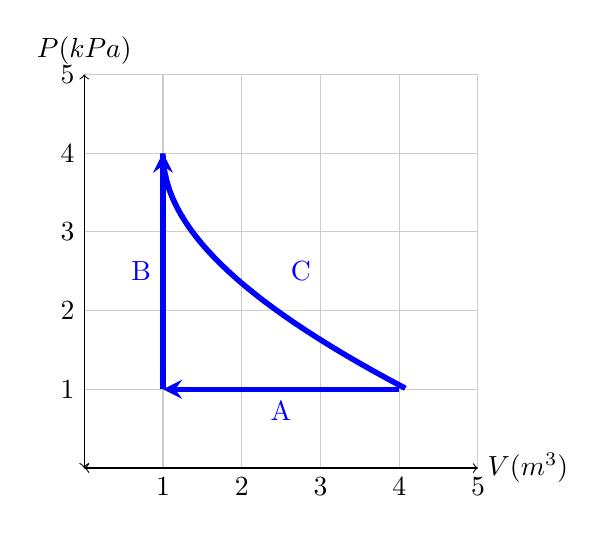
\begin{tikzpicture}
		
		\draw[thin,gray!40] (0,0) grid (5,5);
		\draw[<->] (0,0)--(5,0) node[right]{$V (\si{m^3})$};
		\draw[<->] (0,0)--(0,5) node[above]{$P (\si{kPa})$};
		\draw[line width=2pt,blue,-stealth](4,1) -- (2.5,1) node[below]{A} -- (1,1) ;
		\draw[line width=2pt,blue,-stealth](1,1)-- (1,2.5) node [left] {B} -- (1,4);
		\draw[line width=2pt,blue,-stealth] plot[blue,variable=\t,samples=1000,domain=-33:0] ({16*sec(\t)-15},{4.6*(tan(\t))+4});
		\draw [blue](2.5,2.5) node[right] {C};
		\draw (0,1) node[left] {1};
		\draw (0,2) node[left] {2};
		\draw (0,3) node[left] {3};
		\draw (0,4) node[left] {4};
		\draw (0,5) node[left] {5};
		
		\draw (1,0) node[below] {1};
		\draw (2,0) node[below] {2};
		\draw (3,0) node[below] {3};
		\draw (4,0) node[below] {4};
		\draw (5,0) node[below] {5};		
		
	\end{tikzpicture}

\end{figure}
	


